
\section{削除した原子を色分け表示}
前研究者の岩佐が取り入れた原子の削除操作で,削除された原子の位置を視覚的に把握しやすくするためにおこなった.
図{図:010}は削除の有無で色分けされた原子配置の三面図である.

\begin{figure}[htbp]\begin{center}
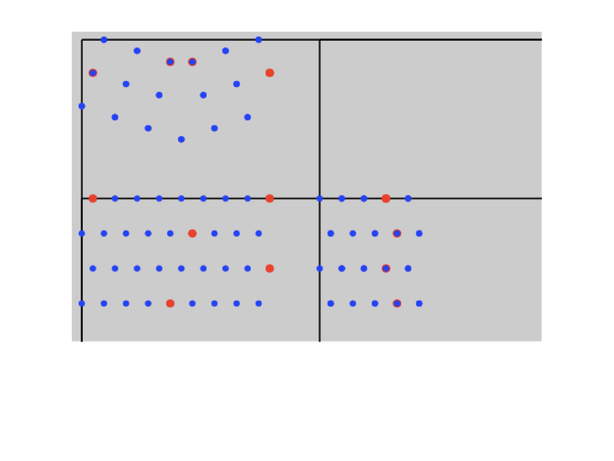
\includegraphics[width=6cm,bb=0 0 442 500]{../figs/./boundary_narita.010.jpg}
\caption{}
\label{default}\end{center}\end{figure}
赤い球が削除された原子に相当する.
viewerで表示することにより,削除された原子の数,並びに各々の配置をすぐに把握することが出来る.

\section{構造緩和による原子移動の表示}
再安定の原子配列にするために構造緩和をおこなう.
構造緩和によって移動した原子の位置を三面図で表示した.

\begin{figure}[htbp]\begin{center}
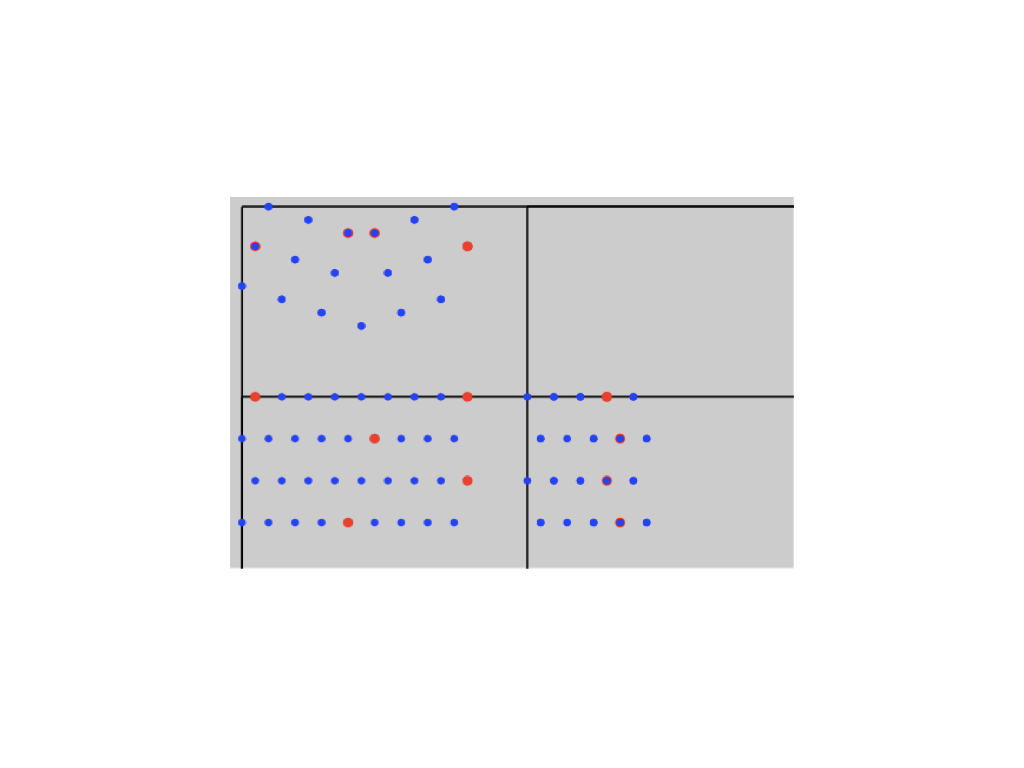
\includegraphics[width=6cm,bb=0 0 442 500]{../figs/./boundary_narita.011.jpg}
\caption{}
\label{default}\end{center}\end{figure}
図中の緑の線が,構造緩和する前とした後の移動した軌道である.

\section{指定したz軸層の白抜き表示}
POSCAR\_2223は4層の原子配列で構成されているため,原子配列を上から見た図,すなわち平面図では,原子同士が重なって配置してしまう.
したがって,指定した層の原子が上から見てどこに位置するのかを視覚的に確認できるために原子の白抜き処理をおこなった.

\begin{figure}[htbp]\begin{center}
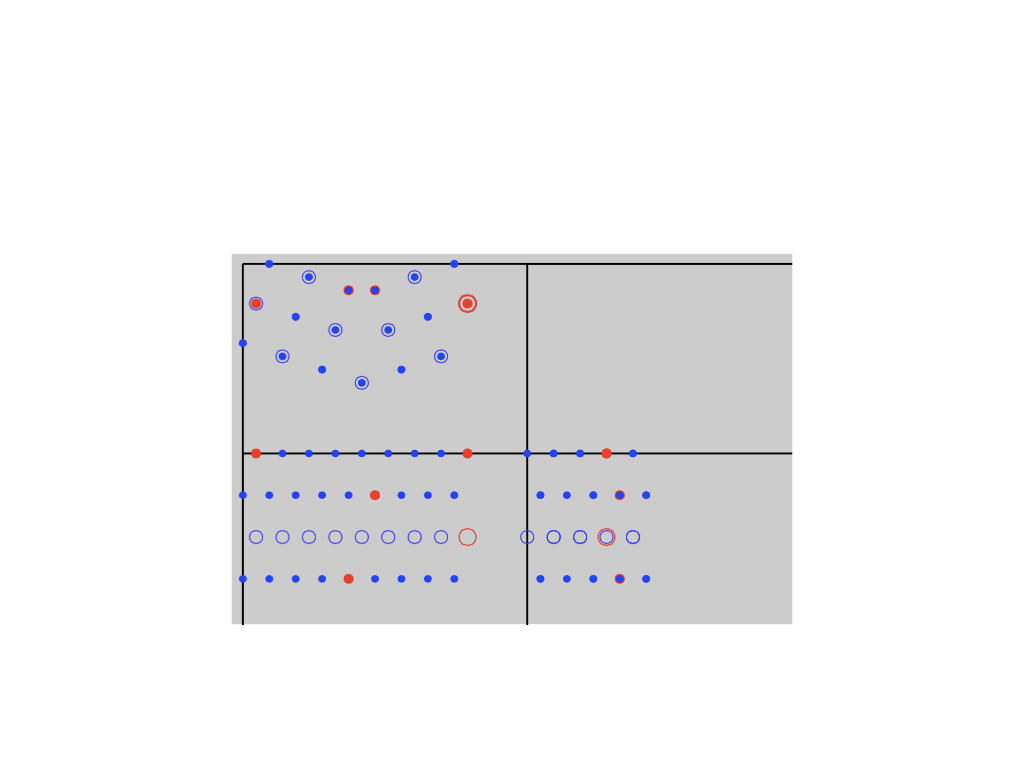
\includegraphics[width=6cm,bb=0 0 442 500]{../figs/./boundary_narita.012.jpg}
\caption{}
\label{default}\end{center}\end{figure}
\section{viewerによる表示の結果}
viewerで原子配列を表示した結果,構造緩和をおこなうためのPOSCARファイルに原子が一つ不足していることが分かった.

\begin{figure}[htbp]\begin{center}
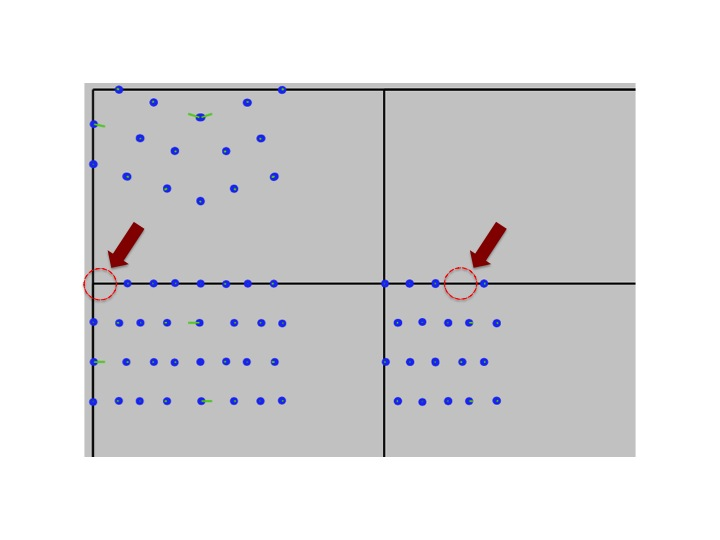
\includegraphics[width=6cm,bb=0 0 442 500]{../figs/./boundary_narita.013.jpg}
\caption{}
\label{default}\end{center}\end{figure}
これまでは,結晶構造描画ソフト"VESTA"を使用していたため,原子の細かい位置が確認できず,原子が不足していることに気がつかなかった.
viewerを使って原子配列を2次元,且つ3方向からの視点で表示したことで,構造緩和をおこなうためのPOSCARファイルに過ちがあったことを発見することができた.

\section{今後の課題}
